%\documentclass[honours,12pt,twoside]{unswthesis}

\usepackage{afterpage}
\usepackage{amsfonts}
\usepackage{amsmath}
\usepackage{amssymb}
\usepackage{amsthm}
\usepackage[english]{babel}
\usepackage{graphicx}
\usepackage{natbib}
\usepackage[utf8]{inputenc}
\usepackage{latexsym}
\usepackage{url}
\usepackage{todonotes}
\usepackage{tikz}
\usepackage{pdfpages}
\usetikzlibrary{arrows}
\usepackage{float}

\usepackage{booktabs}
\renewcommand{\arraystretch}{1.2}


%%%%%%%%%%%%%%%%%%%%%%%%%%%%%%%%%%%%%%%%%%%%%%%%%%%%%%%%%%%%%%%%%
%
%  The following are some simple LaTeX macros to give some
%  commonly used letters in funny fonts. You may need more or less of
%  these
%
\newcommand{\R}{\mathbb{R}}
\newcommand{\Q}{\mathbb{Q}}
\newcommand{\C}{\mathbb{C}}
\newcommand{\N}{\mathbb{N}}
\newcommand{\F}{\mathbb{F}}
\newcommand{\PP}{\mathbb{P}}
\newcommand{\T}{\mathbb{T}}
\newcommand{\Z}{\mathbb{Z}}
\newcommand{\B}{\mathfrak{B}}
\newcommand{\BB}{\mathcal{B}}
\newcommand{\M}{\mathfrak{M}}
\newcommand{\X}{\mathfrak{X}}
\newcommand{\Y}{\mathfrak{Y}}
\newcommand{\CC}{\mathcal{C}}
\newcommand{\E}{\mathbb{E}}
\newcommand{\cP}{\mathcal{P}}
\newcommand{\cS}{\mathcal{S}}
\newcommand{\A}{\mathcal{A}}
\newcommand{\ZZ}{\mathcal{Z}}

%%%%%%%%%%%%%%%%%%%%%%%%%%%%%%%%%%%%%%%%%%%%%%%%%%%%%%%%%%%%%%%%%%%%%
%
% The following are much more esoteric commands that I have left in
% so that this file still processes. Use or delete as you see fit
%
\newcommand{\bv}[1]{\mbox{BV($#1$)}}
\newcommand{\comb}[2]{\left(\!\!\!\begin{array}{c}#1\\#2\end{array}\!\!\!\right)
}
\newcommand{\Lat}{{\rm Lat}}
\newcommand{\var}{\mathop{\rm var}}
\newcommand{\Pt}{{\mathcal P}}
\def\tr(#1){{\rm trace}(#1)}
\def\Exp(#1){{\mathbb E}(#1)}
\def\Exps(#1){{\mathbb E}\sparen(#1)}
\newcommand{\floor}[1]{\left\lfloor #1 \right\rfloor}
\newcommand{\ceil}[1]{\left\lceil #1 \right\rceil}
\newcommand{\hatt}[1]{\widehat #1}
\newcommand{\modeq}[3]{#1 \equiv #2 \,(\text{mod}\, #3)}
\newcommand{\rmod}{\,\mathrm{mod}\,}
\newcommand{\p}{\hphantom{+}}
\newcommand{\vect}[1]{\mbox{\boldmath $ #1 $}}
\newcommand{\reff}[2]{\ref{#1}.\ref{#2}}
\newcommand{\psum}[2]{\sum_{#1}^{#2}\!\!\!'\,\,}
\newcommand{\bin}[2]{\left( \begin{array}{@{}c@{}}
				#1 \\ #2
			\end{array}\right)	}
%
%  Macros - some of these are in plain TeX (gasp!)
%
\newcommand{\be}{($\beta$)}
\newcommand{\eqp}{\mathrel{{=}_p}}
\newcommand{\ltp}{\mathrel{{\prec}_p}}
\newcommand{\lep}{\mathrel{{\preceq}_p}}
\def\brack#1{\left \{ #1 \right \}}
\def\bul{$\bullet$\ }
\def\cl{{\rm cl}}
\let\del=\partial
\def\enditem{\par\smallskip\noindent}
\def\implies{\Rightarrow}
\def\inpr#1,#2{\t \hbox{\langle #1 , #2 \rangle} \t}
\def\ip<#1,#2>{\langle #1,#2 \rangle}
\def\lp{\ell^p}
\def\maxb#1{\max \brack{#1}}
\def\minb#1{\min \brack{#1}}
\def\mod#1{\left \vert #1 \right \vert}
\def\norm#1{\left \Vert #1 \right \Vert}
\def\paren(#1){\left( #1 \right)}
\def\qed{\hfill \hbox{$\Box$} \smallskip}
\def\sbrack#1{\Bigl \{ #1 \Bigr \} }
\def\ssbrack#1{ \{ #1 \} }
\def\smod#1{\Bigl \vert #1 \Bigr \vert}
\def\smmod#1{\bigl \vert #1 \bigr \vert}
\def\ssmod#1{\vert #1 \vert}
\def\sspmod#1{\vert\, #1 \, \vert}
\def\snorm#1{\Bigl \Vert #1 \Bigr \Vert}
\def\ssnorm#1{\Vert #1 \Vert}
\def\sparen(#1){\Bigl ( #1 \Bigr )}

\newcommand\blankpage{%
    \null
    \thispagestyle{empty}%
    \addtocounter{page}{-1}%
    \newpage}
    
%%%%%%%%%%%%%%%%%%%%%%%%%%%%%%%%%%%%%%%%%%%%%%%%%%%%%%%%%%%%%%
%
% These environments allow you to get nice numbered headings
%  for your Theorems, Definitions etc.  
%
%  Environments
%
%%%%%%%%%%%%%%%%%%%%%%%%%%%%%%%

\newtheorem{theorem}{Theorem}[section]
\newtheorem{lemma}[theorem]{Lemma}
\newtheorem{proposition}[theorem]{Proposition}
\newtheorem{corollary}[theorem]{Corollary}
\newtheorem{conjecture}[theorem]{Conjecture}
\newtheorem{definition}[theorem]{Definition}
\newtheorem{example}{Example}
\newtheorem{remark}[theorem]{Remark}
\newtheorem{question}[theorem]{Question}
\newtheorem{notation}[theorem]{Notation}
\numberwithin{equation}{section}

%\begin{document}



\chapter{Magnetic Resonance Imaging and Small Vessel Disease}\label{mri_svd_intro}

An overview of some background knowledge is required to understand the data and the features that are being detected. This chapter introduces the general structure of the brain, MRI and the resulting images, SVD biomarkers, and the existing rating standards.

\section{Structure of the Brain}\label{svd-brain}

The \textit{central nervous system} (CNS) is made up of the brain and spinal chord. Information from throughout the body is communicated via nerves, through the spinal chord, and to the brain. The brain is then tasked with receiving, interpreting and then responding to these signals. The brain itself is the most complex mechanism in the human body, and can be segmented into a number of regions, responsible for different roles. 

The \textit{cerebrum} is the largest part of the brain, forming the outer surface. It is responsible for voluntary actions, senses, thought and memory. It is divided into two hemispheres - left and right, and each hemisphere divides into four lobes:
 \begin{itemize}
	\item The \textit{frontal lobe} is located at the front of the cerebrum. It is responsible for voluntary movement, skills and behaviours, mood and memory.
	\item The \textit{parietal lobe} is situated behind the frontal lobe and is responsible for the senses, including pain, and physical and spacial awareness.
	\item The \textit{temporal lobe} is located at the the side of the cerebrum, and is responsible for for memory and auditory functions, including hearing and speech.
	\item The \textit{occipital lobe} is at the back of the cerebrum, behind the parietal lobe. It is responsible for visual information.
\end{itemize}

% Cerebrum diagram
\begin{figure}[ht]
	\centering
	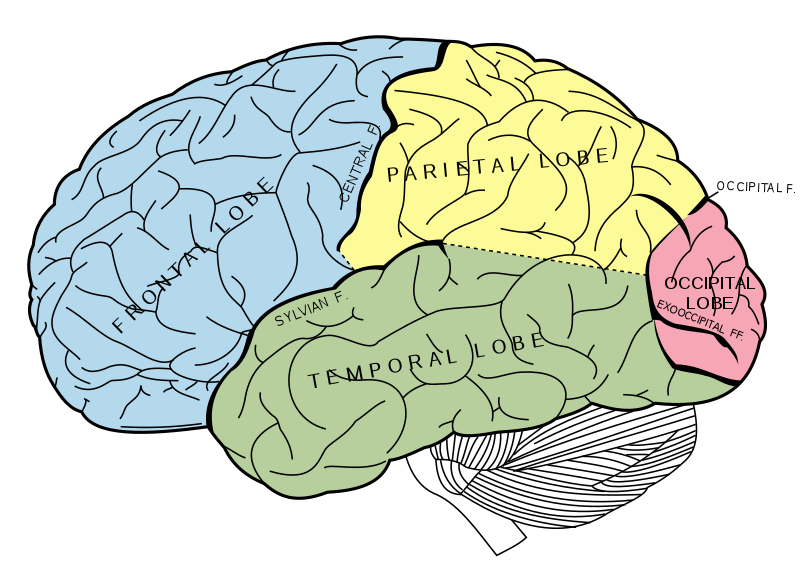
\includegraphics[width=0.8\textwidth]{Images/2_Lobes_of_the_brain_NL.png}
	\caption{The four lobes of the cerebral cortex.}
	\small Image taken from Wikimedia Commons: \url{'Gray728.svg'}
\end{figure}

% Gray vs white matter diagram
\textbf{[Grey vs white matter diagram]}

% Basal Ganglia
\begin{figure}[ht]
	\centering
	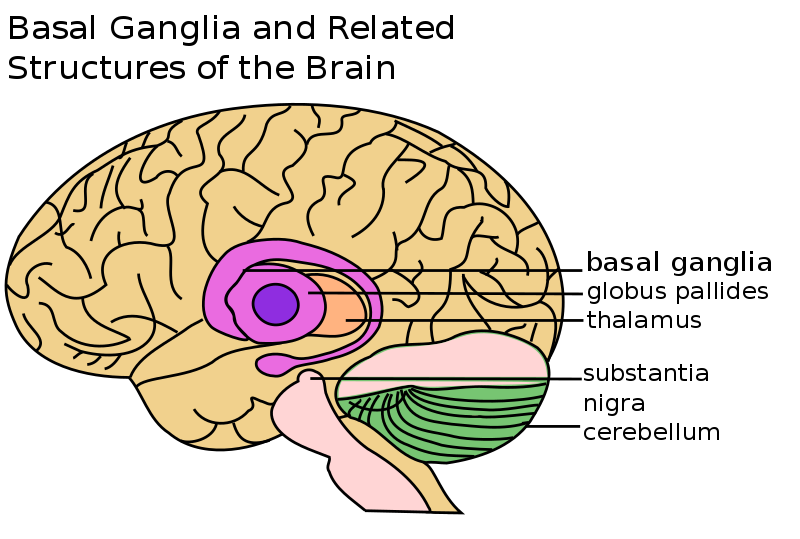
\includegraphics[width=0.8\textwidth]{Images/2_Basal_Ganglia_and_Related_Structures.png}
	\caption{The basal ganglia and other related structures.}
	\small Image taken from Wikimedia Commons: \url{'Basal_Ganglia_and_Related_Structures.svg'}
\end{figure}


The outer surface of the brain consists of a layer of neurons referred to as \textit{grey matter}. This layer has a thickness of around 4mm, and much of the brain processes occur here. Grey matter also occurs in the cerebellum, brainstem and within the spinal chord.

Underneath the grey matter is a network of fibres that connects these grey matter neurons together. Collectively, they form the \textit{white matter}. 

At the centre of the brain, the main structures include the thalamus, hypothalamus and pituitary gland. Of particular interest are a group of structures that form the \textit{basal ganglia}. This region of the brain is responsible for voluntary movement and learning; and exhibits more numerous instances of lacunes and perivascular spaces.

At the base of the brain lies the cerebellum and brain stem. These are responsible for coordination and the transmission of nerve communications respectively.

Within the skull, the brain sits in \textit{cerebral spinal fluid} (CSF). This fluid can flow between the ridges  at the surface of the brain, to be found filling gaps, such as perivascular spaces, throughout the brain matter.


\section{Magnetic Resonance Imaging}\label{svd-MRI}

\textit{Magnetic Resonance Imaging }(MRI) is a radiological technique that uses magnetic fields and radio waves to generate greyscale images of organs inside the body. The two most common images produced are referred to as \textit{T1-weighted} and \textit{T2-weighted} images.

% Image comparisons
\begin{figure}[ht]
	\centering
	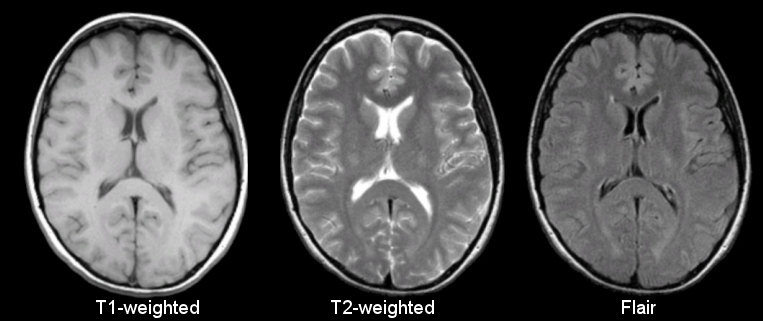
\includegraphics[width=\textwidth]{Images/2_t1_t2_flair.jpg}
	\caption{A comparison of T1, T2 and FLAIR images.}
	\small Image taken from \cite{Preston2006}
\end{figure}

T1-weighted images are bright in regions with high fat content, such as white matter, and are dark in regions with high water content, usually CSF.

In contrast, T2-weighted images are bright in regions with high fat and water content. This can make it easier to spot abnormalities.

\textit{FLuid-Attenuated Inversion Recovery} (FLAIR) is another commonly used imaging sequence. It is similar to that of T2, except that CSF remains dark. This allows for easier identification of abnormalities against CSF.

% T1, T2 and FLAIR images

MRI scan data is made up of numerous 2D slices, that together form a three dimensional volume. The data itself is stored in a variety of formats, some frequent file types include Analyze, Nifti, Mine and Dicom. The resolution of an MRI scanner is higher than that of other scans, such as CT scanning, so is frequently preferred for neurological and cancer studies.

\section{Biomarkers of Small Vessel Disease}\label{svd-markers}

In the analysis of MRI scans for SVD, there are a number of biomarkers that clinicians look for. Two of these markers include lacunes and perivascular spaces. Though appearing similar in MRI, their origins greatly contrast each other, and so there is the need to differentiate between them.

Prior to 2013, there were no official guidelines for the identification of these events. There were several studies attempting to establish guidelines for consistency \cite{PotterGillian2015CPSV, AdamsH.H.Hieab2013RMfD}, however these methods tended to focus on only specific events rather than SVD biomarkers in general.

In addition, much of the terminology surrounding some biomarkers was inconsistent. For instance, perivascular spaces are also frequently referred to as Virchow-Robin spaces\cite{WardlawJ.M.2013Nsfr, AdamsH.H.Hieab2013RMfD}.

As a result, the STRIVE criterion \cite{WardlawJ.M.2013Nsfr} were put into place to standardise the terminology and definitions surrounding SVD biomakers.

% Images of lacunes and perivascular spaces from STRIVE
\begin{figure}[ht]
	\centering
	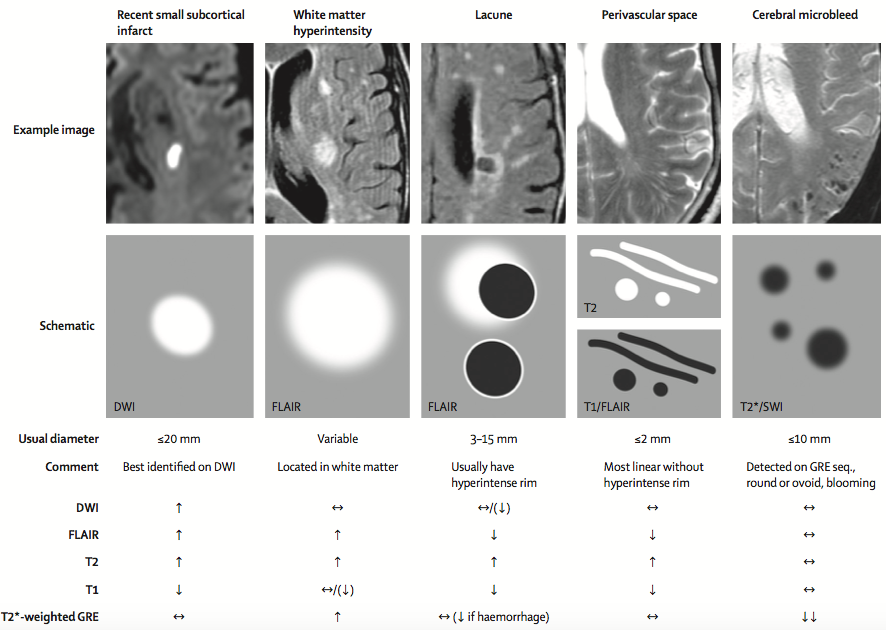
\includegraphics[width = \textwidth]{Images/2_STRIVE.png}
	\caption{STRIVE criterion and MRI examples.}
	\small Image taken from \cite{WardlawJ.M.2013Nsfr}
\end{figure}

Lacunes are defined as a form of small brain cavity. They usually appear without symptoms, and are frequently found in the scans of elderly. When present, they indicate a heightened risk of stroke and dementia \cite{VanDerFlierM.Wiesje2005SVDa, BenjaminJ.Philip2018LIbN}. In MRI, lacunes appear round, with a diameter between 3mm and 15mm. As they are filled with fluid, they tend to give off a darker signal intensity, similar to that of CSF. Lacunes also have a tendency to occur in regions of white matter hyperintensity, so will frequently have a hyperintense rim in FLAIR imaging.

Perivascular spaces are extensions of the fluid space surrounding blood vessels through the brain. They are generally microscopic but can become enlarged with age, and often appear alongside other SVD biomarkers such as lacunes and white matter hyperintensities. As they are fluid-filled, perivascular spaces also take on a similar signal intensity to CSF. They are found running parallel to vessels, and are generally found under 3mm in diameter. As they are tubular, they can be identified by appearing circular cross-sectionally, but oblong when viewed in parallel to the vessels.

Other biomarkers of interest include white matter hyperintensities, cerebral microbleeds, recent small subcortical infarcts and brain atrophy. 

White matter hyperintensities are regions of hyperintensity shown in T2-weighted imaging. They also appear in T1-weighted images, but are hypointense, though not as dark as CSF. Their cause is not well understood.

Cerebral microbleeds are blooming regions of microscopic bleeding, around 2-5mm in diameter, though they can be larger. They are not visible on T1-weighted, T2-weighted and FLAIR images, and are instead found in T2*-imaging - constructed as a combination of T2-imaging and inhomogeneities in the magnetic field during scanning. 

Recent Small subcortical infarcts, also called lacunar strokes, are the cause of 25\% of ischaemic (oxygen starved) strokes \cite{WardlawJ.M.2013Nsfr}. There are regions of recent oxygen deprivation that has resulted in dying cells. These lesions are usually less than 20mm in diameter. 

Brain atrophy refers to the reduction of brain matter, not restricted to particular regions of the brain. It can be identified by the increase in CSF volume in T1-weighted, T2-weighted and FLAIR imaging.


\section{Existing Rating Methods}\label{svd-rating}

Without a biopsy for confirmation, the identification of SVD biomarkers relies on MRI. Current rating methods involve trained observers examining MRI slice by slice. They then identify any lesions or points of interest in conjunction with the STRIVE criterion \cite{WardlawJ.M.2013Nsfr}. Though the criterion helped to standardise the definition of lacunes and perivascular spaces, their appearances are still highly similar, and so difficult to distinguish. As a result, manual rating has been found to be highly inconsistent \cite{PotterGillian2015CPSV}. 

In addition, the manual rating process is also time consuming. The checking and logging of an individual scan can take over 10 minutes.

It is only recently that machine learning algorithms have begun to improve the rating process. Dou et al. \cite{DouQ.2016ADoC} released a machine learning algorithm for the detection of cerebral microbleeds. This algorithm exhibited a sensitivity of 93.16\%, with an average of 2.74 false positives per slice. 

Ghafoorian et al. \cite{GhafoorianM.2017Dml3} developed a machine learning algorithm for the automated detection of lacunes. This algorithm was able to achieve a sensitivity of 97.4\%, with 0.13 false positives per slice. \textbf{This algorithm will be discussed further in Section.}

%%%%%%%%%%%%%%%%%%%%%%%%%%%%%%%%%%%%%%%%%%%%%%%%%%%%%%%%%%%%%%%%%%%%%%%%%%

%\clearpage

\addcontentsline{toc}{chapter}{References}

\bibliographystyle{apalike}
\bibliography{bibliography.bib}

%\bibliographystyle{apacite}
%\bibliography{mybib.bib}

